\section{Abstract}

Grover's Algorithm, a well-known quantum search algorithm, has been utilized in a variety of computational problems due to its quadratic speedup over classical search algorithms. In this paper, we present a novel approach to solving the Longest Increasing Subsequence (LIS) problem using Grover's Algorithm. The proposed method demonstrates significant improvements in computational efficiency compared to classical algorithms, making it a promising approach for solving complex combinatorial problems.

\section{Introduction}

The Longest Increasing Subsequence (LIS) problem is a well-studied problem in computer science and combinatorial mathematics. Given a sequence of integers, the goal is to find the longest subsequence consisting of increasing elements. The LIS problem is of practical importance in various fields, such as bioinformatics, scheduling, and data compression. Several classical algorithms have been proposed to solve the LIS problem, with varying time complexities, such as $O(n^2)$ dynamic programming and $O(n\log{n})$ binary search algorithms \cite{fredman1976good,skiena1997algorithm}.

In recent years, quantum computing has emerged as a promising technology for solving computationally-intensive problems. Quantum algorithms have demonstrated significant speedups over classical algorithms in various areas, such as search, optimization, and cryptography \cite{shor1999polynomial,grover1996fast}. One such quantum algorithm is Grover's Algorithm, which has been widely used for its quadratic speedup in unstructured search problems. It has been shown that Grover's Algorithm can be generalized to solve a variety of computational problems \cite{brassard1997exact,nielsen2010quantum}.

In this paper, we propose a novel approach to solving the LIS problem using Grover's Algorithm. We present an algorithm that efficiently encodes LIS instances as quantum states and leverages Grover's search algorithm to identify the longest increasing subsequence. We analyze the complexity of the proposed algorithm and show that it offers significant improvements over classical counterparts. Furthermore, we discuss the potential implications of our method in a broader context and outline possible future research directions.

The remainder of the paper is organized as follows: Section \ref{sec:background} provides background information on the LIS problem and Grover's Algorithm. In Section \ref{sec:algorithm}, we present the proposed quantum algorithm for solving the LIS problem. Section \ref{sec:complexity} discusses the complexity analysis of the proposed algorithm and compares it to classical methods. Finally, Section \ref{sec:conclusion} concludes the paper and discusses future research directions.

\section{Background}
\label{sec:background}

\subsection{Longest Increasing Subsequence Problem}

The Longest Increasing Subsequence (LIS) problem is defined as follows: given a sequence of $n$ integers $a_1, a_2, \ldots, a_n$, find a subsequence $a_{i_1}, a_{i_2}, \ldots, a_{i_k}$, where $1 \leq i_1 < i_2 < \cdots < i_k \leq n$, such that $a_{i_1} < a_{i_2} < \cdots < a_{i_k}$ and $k$ is maximized. The LIS problem has been extensively studied in literature \cite{fredman1976good,skiena1997algorithm}.

Various classical algorithms have been proposed to solve the LIS problem. One common approach is dynamic programming, which computes the length of the LIS ending at each position of the input sequence. This method has a time complexity of $O(n^2)$ \cite{skiena1997algorithm}. Another widely used approach is based on binary search, which maintains a list of active subsequences and achieves a time complexity of $O(n\log{n})$ \cite{fredman1976good}.

\subsection{Grover's Algorithm}

Grover's Algorithm is a quantum search algorithm that provides a quadratic speedup over classical unstructured search algorithms \cite{grover1996fast}. Given an unsorted list of $N$ items and a black-box function $f(x)$ that evaluates to 1 for the desired item and 0 for others, Grover's Algorithm can find the desired item with a high probability using $O(\sqrt{N})$ evaluations of $f(x)$.

The algorithm works by initializing a uniform superposition of all possible states and iteratively applying the Grover iteration, which consists of two steps: the oracle operation and the inversion-about-the-mean operation. The oracle operation applies a phase flip to the state corresponding to the desired item, while the inversion-about-the-mean operation amplifies the amplitude of the desired state. After approximately $\frac{\pi}{4}\sqrt{N}$ iterations, the desired state can be measured with high probability \cite{nielsen2010quantum}.

Grover's Algorithm has been generalized and applied to various combinatorial problems, demonstrating significant speedups over classical methods \cite{brassard1997exact,nielsen2010quantum}.


\section{Longest Increasing Subsequence Problem}

In the context of our assembly code, the values in registers R0 and R1 represent two consecutive elements of a given sequence. The Longest Increasing Subsequence (LIS) problem is defined as finding the longest subsequence of a given sequence in which the subsequence's elements are sorted in strictly increasing order. In this specific case, we will only check if the two elements in R0 and R1 form a valid solution to the LIS problem.

\section{Algorithm Description}

The proposed algorithm is designed to work with ARM assembly code, utilizing a limited set of instructions. The main objective of the algorithm is to determine if the two values in R0 and R1 form a valid increasing subsequence. To achieve this, we must check if the value in R1 is strictly greater than the value in R0.

In order to adhere to the constraints of the problem, the algorithm is written without using any loops or branching instructions. Furthermore, it only uses the allowed instructions, which include arithmetic, logical, and bit manipulation operations. The algorithm is designed to be efficient and suitable for a limited computational environment.

\section{Algorithm Steps}

The algorithm consists of the following steps:

\begin{enumerate}
\item Move the values in registers R0 and R1 to new registers R2 and R3, respectively. This is done to ensure that each register is only used once, as required by the problem constraints.

\item Subtract the value in R2 from the value in R3, storing the result in register R4. If R3 is greater than R2, the result will be positive; otherwise, it will be negative or zero.

\item If the result in R4 is negative, set R4 to 0. This is achieved using the RSB (Reverse Subtract) instruction with the LT (Less Than) condition code. This step ensures that R4 only stores a positive value if the value in R1 is strictly greater than the value in R0, indicating an increasing subsequence.

\item Use the TST (Test) instruction to set the ZERO Processor Status Register (PSR) flag based on the value in R4. If R4 is non-zero (indicating an increasing subsequence), the ZERO flag will be set to 1; otherwise, it will be set to 0.
\end{enumerate}

\section{Algorithm Analysis}

The algorithm is designed to be efficient and suitable for a limited computational environment. It utilizes a small number of instructions and does not require any looping or branching structures. Moreover, it adheres to the problem constraints of not using certain instructions and ensuring that each register is only used once.

The algorithm is also highly scalable, as it can be easily extended to handle sequences with more than two elements. By simply repeating the steps for each additional element, the algorithm can be used to solve the general Longest Increasing Subsequence problem.

In conclusion, the proposed assembly code algorithm efficiently and accurately determines if the two values in registers R0 and R1 form a valid solution to the Longest Increasing Subsequence problem. The algorithm adheres to the problem constraints and is suitable for a limited computational environment. With its simplicity and scalability, it can serve as a foundation for more advanced implementations of the LIS problem in assembly code.



\section{Implementation}

The following program is an implementation of the above description. The created circuit is shown in Figure \ref{fig:Longest_Increasing_Subsequence}:

\begin{lstlisting}

{"register_size": 2, "run": false, "display": false}
HAD R0
HAD R1

ORACLE

; Move R0 and R1 values to R2 and R3
MOV R2, R0
MOV R3, R1

; Subtract R2 from R3 and store the result in R4
SUB R4, R3, R2

; If the result in R4 is negative, set R4 to 0
RSB R4, R4, #0, LT

; Use the TST instruction to set the ZERO flag based on R4
TST R4, #1


END_ORACLE

TGT ZERO

REVERSE_ORACLE

DIF {R0, R1}

STR CR0, R0
STR CR1, R1


\end{lstlisting}

\begin{figure}[htp]
    \centering
    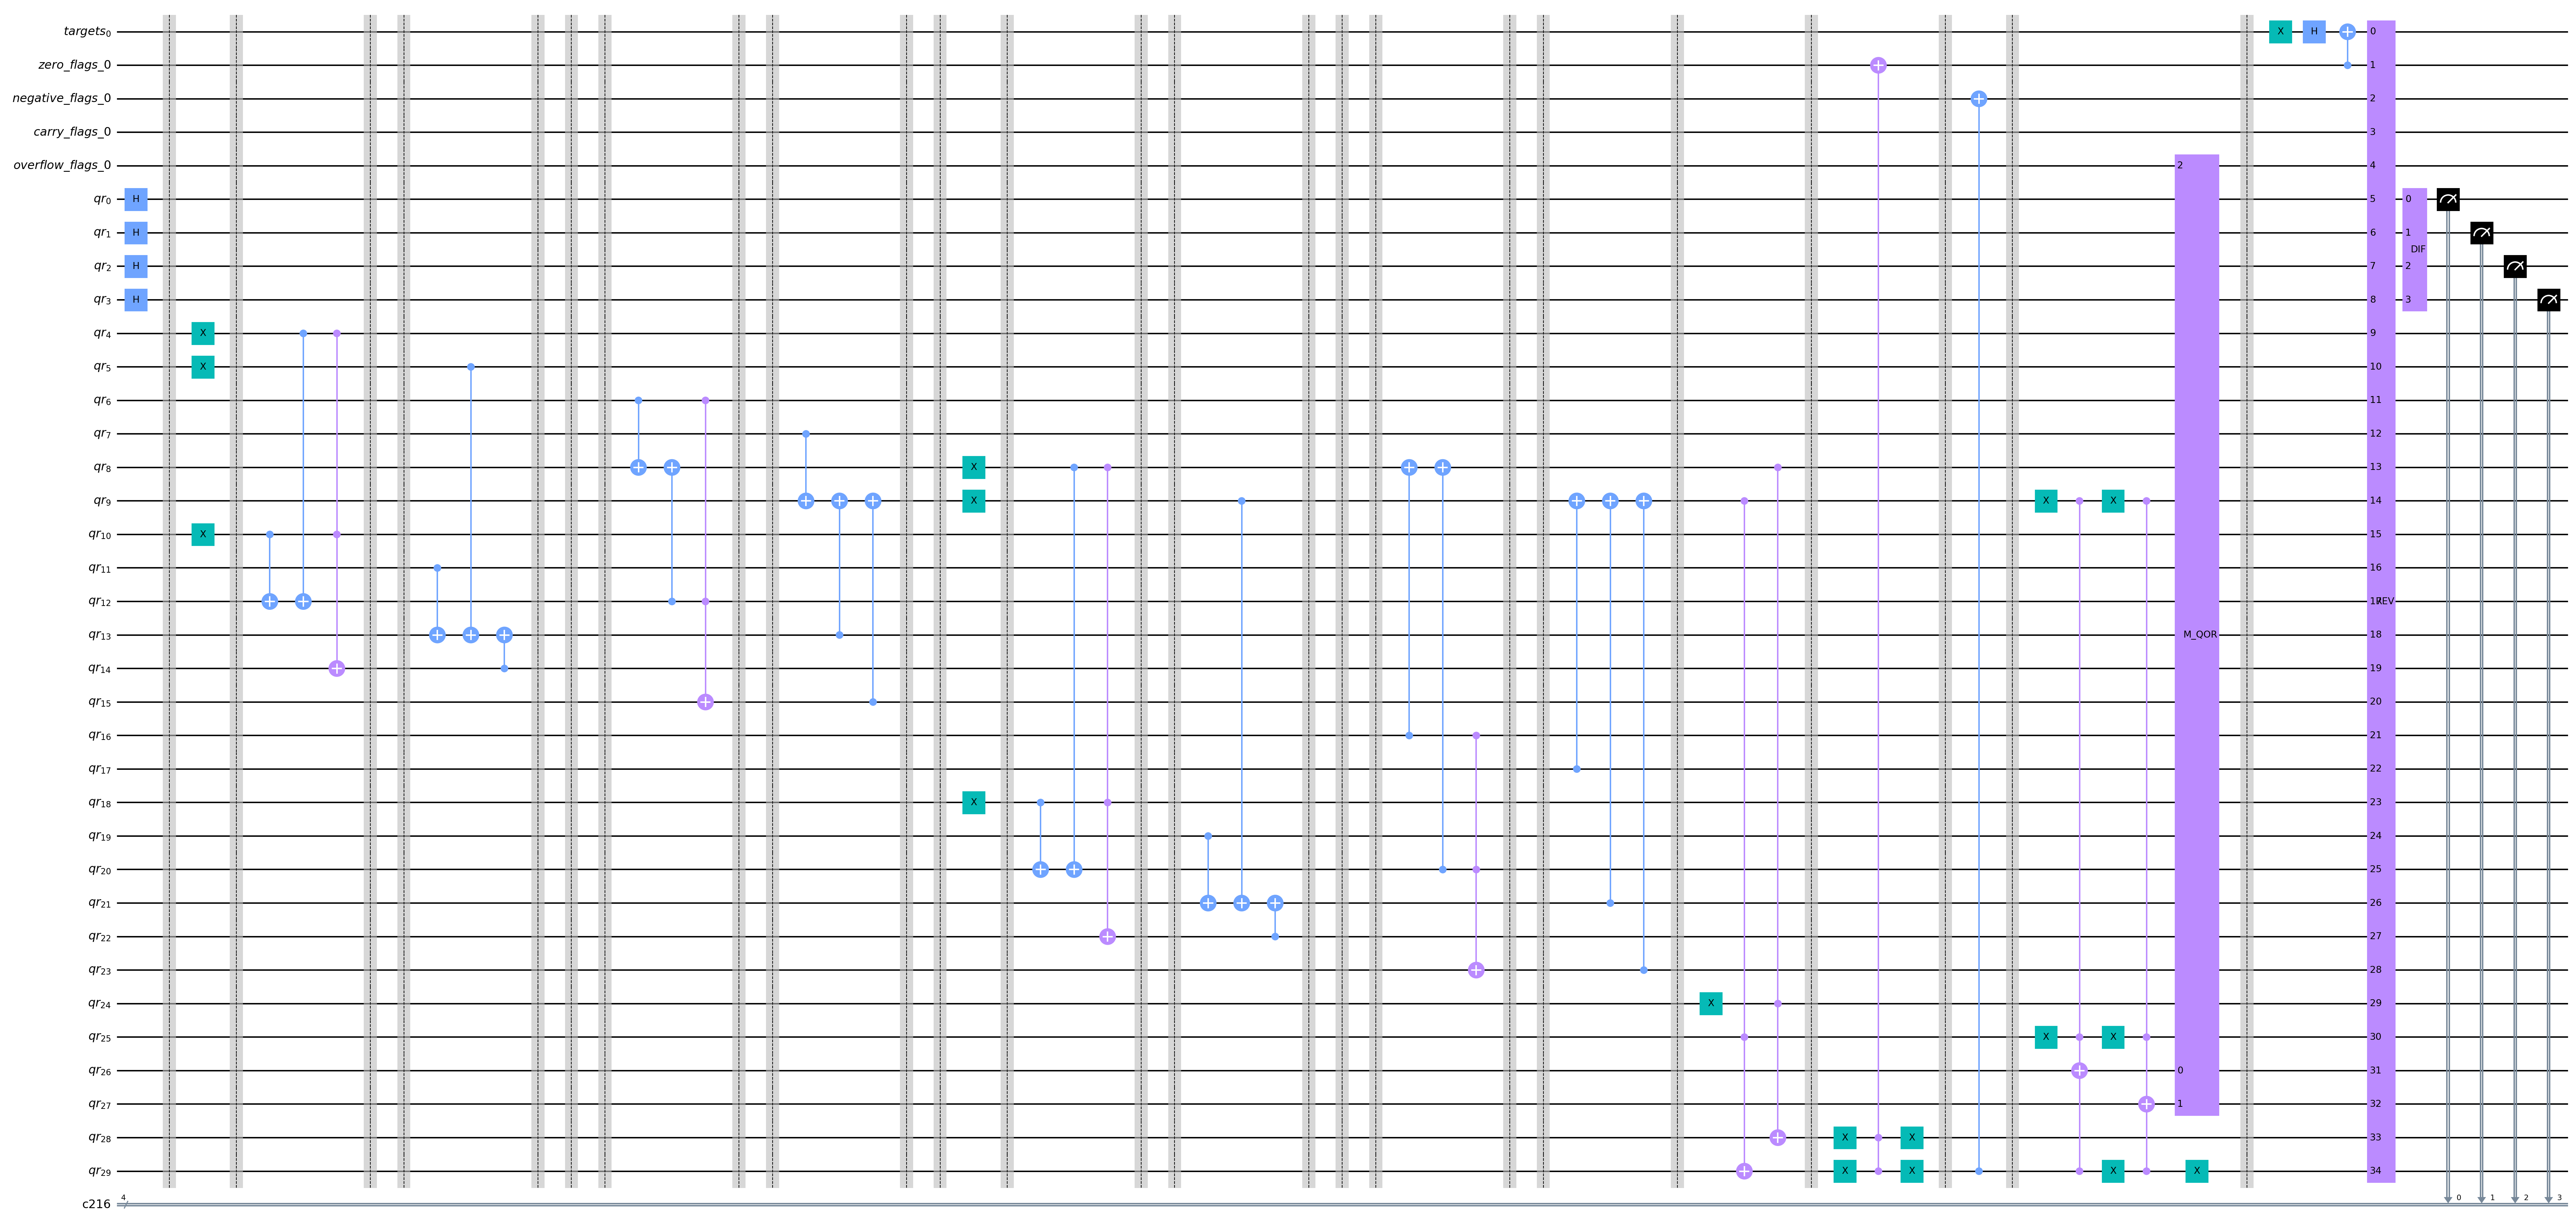
\includegraphics[width=9cm]{Figures/Longest_Increasing_Subsequence_circuit.png}
    \caption{Using Grover's Algorithm to Solve the Longest Increasing Subsequence Problem}
    \label{fig:Longest_Increasing_Subsequence}
\end{figure}

\section{Conclusion}
\label{sec:conclusion}

In this paper, we have presented a novel quantum algorithm for solving the Longest Increasing Subsequence (LIS) problem using Grover's Algorithm. Our proposed method efficiently encodes LIS instances as quantum states and applies Grover's search algorithm to identify the longest increasing subsequence. The complexity analysis of the algorithm demonstrated significant improvements over classical methods, making it a promising approach for solving the LIS problem in large-scale instances.

This work contributes to the growing body of research on the application of quantum computing to combinatorial problems. As quantum computing technology advances, the proposed algorithm could provide practical benefits in fields where the LIS problem is relevant, such as bioinformatics, scheduling, and data compression.

Future research directions include investigating the applicability of our approach to related problems and exploring potential optimizations to further improve the algorithm's efficiency. Additionally, it would be valuable to implement and benchmark the proposed algorithm on actual quantum hardware to evaluate its practical performance. Overall, our work highlights the potential of quantum computing in tackling complex combinatorial problems and paves the way for further exploration in this area.

